\documentclass[11pt]{beamer}
\usetheme[
  workplace=fi,
]{MU}

\usepackage[utf8]{inputenc}
\usepackage[czech]{babel}
\usepackage[T1]{fontenc}
\usepackage{amsmath}
\usepackage{amsfonts}
\usepackage{amssymb}
\usepackage{amsthm}
\usepackage{graphicx}
\usepackage{algpseudocode}
\usepackage{listings}
\usepackage{pgf}
\usepackage{tikz}
%\usepackage[boxruled,vlined,linesnumbered]{algorithm2e}
%\usepackage{algorithm2e}
%\usepackage{hyperref}
\usetikzlibrary{arrows,automata}

%\resetcounteronoverlays{algocf}

\author{Jan Tušil}
\title{Context-Sensitive Dynamic Partial Order Reduction}
%\setbeamercovered{transparent} 
%\setbeamertemplate{navigation symbols}{} 
%\logo{} 
%\institute{} 
%\date{} 
%\subject{} 

\newtheorem{dfn}{Definice}
\newtheorem{tvrzeni}{Tvrzení}

\begin{document}

\begin{frame}
\titlepage
\end{frame}

%\begin{frame}
%\tableofcontents
%\end{frame}

\tikzset{
    no highlight/.style={fill=blue},
    highlight/.style={fill=red}
}

% Jak to celé bude?
% Nejprve POR obecně,
% potom Source-DPOR,
% potom Context-Sensitive Source-DPOR.

% Řekněme, že máme program se dvěma procesy, p a q,
% a zajímá nás, v jakých stavech může tento program skončit.
% Výpočetní strom tohoto programu vypadá takto:
% Dejme tomu, že máme bezstavový model checker,
% tedy model checker, který si nepamatuje navštívené stavy, který již opustil.
% Úplně jednoduchý model checker sestoupí z iniciálního stavu přes p1
% a přes q1 do finálního stavu, pak backtrackuje zpět do iniciálního stavu a odtud sestoupí
% pro změnu přes q1 a p1 do druhého (vlastně toho samého) terminálního stavu.
%
% Trošku chytřejší model checker by si všiml , že instrukce p1 a q1 jsou nezávislé,
% tedy že se navzájem nevypnou ani nezapnou a že jsou komutativní, a druhou sekvenci již nebudou zkoumat.
\begin{frame}[fragile]{Example 1}
\begin{semiverbatim} \small
p: x := 3    q: y := 4
\end{semiverbatim}
\begin{tikzpicture}[>=stealth,node distance=2.0cm,auto]
    \node[state]  (I)                      {$(0,0)$};
    \node[state]                    (p1) [below left of = I] {$(3,0)$};
    \node[state]                    (q1) [below right of = I] {$(0,4)$};
    \node[state]                    (p1q1) [below of = p1] {$(3,4)$};
    \node[state]                    (q1p1) [below of = q1] {$(3,4)$};
    \draw[->] (I) to node{$p_1$} (p1);
    \draw[->] (p1) to node{$q_1$} (p1q1);
    \draw[->] (I) to node{$q_1$} (q1);
    \draw[->] (q1) to node{$p_1$} (q1p1);
\end{tikzpicture}
\end{frame}

% Zde jsou instrukce p1 a q1 závislé, protože obecně nekomutují.
% Model checker tedy musí prozkoumat oba běhy.
\begin{frame}[fragile]{Example 2}
\begin{semiverbatim} \small
p: x := 3    q: y := x
\end{semiverbatim}
\begin{tikzpicture}[>=stealth,node distance=2.0cm,auto]
    \node[state]  (I)                      {$(0,0)$};
    \node[state]                    (p1) [below left of = I] {$(3,0)$};
    \node[state]                    (p1q1) [below of = p1] {$(3,3)$};
    \node[state]                    (q1) [below right of = I] {$(0,0)$};    
    \node[state]                    (q1p1) [below of = q1] {$(3,0)$};
    \draw[->] (I) to node{$p_1$} (p1);
    \draw[->] (p1) to node{$q_1$} (p1q1);
    \draw[->] (I) to node{$q_1$} (q1);
    \draw[->] (q1) to node{$p_1$} (q1p1);
\end{tikzpicture}
\end{frame}

% Tady máme úplně stejný program, ale spouštěný z jiného iniciálního stavu.
% Přestože instrukce p1 a q1 obecně nekomutují, v situaci, kdy proměnná x již má
% hodnotu 3, komutují. Tyto instrukce jsou tedy obecně závislé, ale ve vhodném kontextu
% nezávislé. Tedy opět zde stačí prozkoumat pouze jeden běh.
\begin{frame}[fragile]{Example 3}
\begin{semiverbatim} \small
p: x := 3    q: y := x
\end{semiverbatim}
\begin{tikzpicture}[>=stealth,node distance=2.0cm,auto]
    \node[state]  (I)                      {$(3,1)$};
    \node[state]                    (p1) [below left of = I] {$(3,1)$};
    \node[state]                    (p1q1) [below of = p1] {$(3,3)$};
    \node[state]                    (q1) [below right of = I] {$(3,3)$};    
    \node[state]                    (q1p1) [below of = q1] {$(3,3)$};
    \draw[->] (I) to node{$p_1$} (p1);
    \draw[->] (p1) to node{$q_1$} (p1q1);
    \draw[->] (I) to node{$q_1$} (q1);
    \draw[->] (q1) to node{$p_1$} (q1p1);
\end{tikzpicture}
\end{frame}

%%TODO do hezciho obrazku
%%
%% výpočetní krok
%%             |
%%           vvvvvv
%% [ x := 5; y := x; z++ ]
%% ^^^^^^^^^^^^^^^^^^^^^^^
%% Výpočetní posloupnost
%\begin{frame}{Pojmy}
%%\begin{itemize}
%%\item Krok výpočtu
%%\end{itemize}
%\end{frame}


%\begin{frame}
%\begin{itemize}
%\item Od naivního k Source-POR
%\item Od Source-POR k Context-Sensitive (Source-) POR
%\end{itemize}
%\end{frame}

% Běhy jsou vlastně linearizace relace Happens-Before?
\begin{frame}[fragile]{Happens-Before}
\begin{columns}

\begin{column}{0.5\textwidth}
Program
\begin{semiverbatim} \small
p: write(x);
q: read(y); read(x);
r: read(z); read(x);
\end{semiverbatim}

\onslide<5->
Jaké jsou jiné běhy se stejnou Happens-Before relací?


\onslide<6->

Není ale třeba je zkoumat.

\end{column}
\begin{column}{0.5\textwidth}
\pause
Konkrétní běh:
\begin{semiverbatim} \small
p1: write(x);
q1: read(y);
q2: read(x);
r1: read(z);
r2: read(x);
\end{semiverbatim}
\pause
Happens-Before tohoto běhu:
\pause
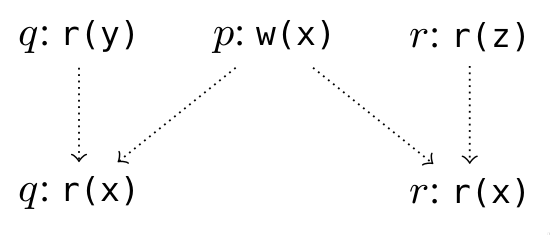
\includegraphics[width=0.9\linewidth]{img/hb1.png}
\end{column}
\end{columns}
\end{frame}


\begin{frame}[fragile]{Notace}
\begin{algorithmic}
\pause \State \textbf{val} Event $ \gets $ Process $ \times \mathbb{N}$
\pause \State \textbf{val} s : State \pause \Comment{Iniciální stav}
\pause \State \textbf{val} s[\_] : Trace -> State \pause \Comment{Stav, do něhož doběhne stopa z s}
\pause \State \textbf{val} enabled : State -> Set<Process>
\pause \State \textbf{var} Sleep : Trace -> Set<Trace> \pause \Comment{Navazující stopy jež netřeba řešit}
\pause \State \textbf{var} backtrack : Trace -> Set<Process>
\pause \State \textbf{val} dom : Trace -> Set<Event>
\end{algorithmic}
\end{frame}


% Idea za Source DPOR: DFS, u každého vrcholu na zásobníku si držím
% seznam hran, které ještě musím projít, a taky seznam, které už projít nemusím.
% Místo abych si ale seznam hran/procesů na projití vytvořil hned při vstupu do uzlu,
% průběžně je tam přidávám, jak zjišťuji, které hrany jsou kolizní.
% Protože není-li kolizní, mohu ji provézt na konci aktuální cesty.
\begin{frame}[fragile]{Source DPOR (1)}

% TODO typy. sleep: ExecSequence
% Btw ExecutionStep je reprezentovan jmenem procesu/vlakna
\begin{algorithmic} \small
%\State \textbf{var} enabled : State -> Set<Process>
%\State \textbf{var} backtrack : Trace -> Set<Process>
%\State \textbf{var} Sleep : Trace -> Set<Trace>
\Function{ExploreSource}{$E$ : Trace, $Sleep$ : Set<Trace>}
  \State $sleep(E) \gets Sleep$
  \State \textbf{choose process} $p \in \textit{enabled}(s[e]) \setminus \textit{Sleep}$
  \textbf{or} \Return
  \State $\textit{backtrack}(E) \gets \{ p \}$;
  
  \While{$\exists p \in \textit{backtrack}(E) \setminus \textit{sleep}(E)$}
    \State \Call{DetectRacesSource}{$E$, $p$}  
    \State $\textit{Sleep}^\prime \gets \{ v \mid v \in \textit{sleep}(E) \land E \vDash p \diamond v \}$
    \State \Call{Explore}{$E.p$, $Sleep^\prime$}
    \State $\textit{sleep}(E) \gets \textit{sleep}(E) \cup \{ p \}$

    %\uncover<3>{\State $z \gets 2$}

  \EndWhile  
\EndFunction
\end{algorithmic}
\end{frame}

% Detekuje konfliktní události na cestě E
\begin{frame}{Source DPOR (2)}

\begin{algorithmic} \small
\Function{DetectRacesSource}{E : Trace, p: Process}
\State \textbf{val} $e_p$ : Event $ \gets \textit{next}_E(p)$
%\ForAll{$e \in \textit{dom}(E)$} \textbf{such that} $e \precsim_{E.p} pe f$
\ForAll{$e \in \textit{dom}(E)$ \textbf{such that} $e$ is in reversible race with $e_p$}
  \State \textbf{val} $E^\prime \gets \textit{prefixBefore}(E, e)$ \Comment{does not include $e$}
  \State \textbf{val} $v : \textsf{Trace} \gets \textit{indepSuffixAfter}(e, E).p$ \Comment{does not include $e$}
  \only<1>{\If{the first event of $v$ is not in $\textit{backtrack}(E^\prime)$}
    \State add it there
  \EndIf}
  % More general version
  \only<2>{\If{$I_{E^\prime}(v) \cap \textit{backtrack}(E^\prime) \not = \emptyset$}
    \State add some $q^\prime \in I_{E^\prime}(v)$ to $\textit{backtrack}(E^\prime)$
  \EndIf}
\EndFor
\EndFunction
\end{algorithmic}
\uncover<2>{Výraz $I_{E^\prime}(v)$ označuje procesy,
které mají v posloupnosti $v$ nějakou událost,
která nenastává po (ve smyslu happens-before) žádné jiné události ve $v$.}
\end{frame}

\begin{frame}[fragile]{Source DPOR - příklad}
\begin{semiverbatim}
p: write(x);
q: read(y); read(x);
r: read(z); read(x);
\end{semiverbatim}
\pause
Na tabuli
\end{frame}

\begin{frame}[fragile]{Source DPOR není citlivé na kontext}
\begin{semiverbatim}
p: write(x = 5);
q: write(x = 5);
r: read(x)
\end{semiverbatim}
\pause
Na tabuli
\end{frame}


% Proč potřebuji pojmy? Abych definoval happens-before a Mazurkiewiczovu stopu

% Hmm, optimální DPOR nestaví na žádné konkrétní HB relaci,
% ale na abstraktní HB - prostě relace (resp. funkce ze stop na relaci)
% splňující nějaké požadavky.

% Mohli bychom říci, že naše zvolená HB relace není context-sensitivní,
% protože instrukce musí být nezávislé úplně. Ale ukazuje se, že 
% každá HB relace povolená algoritmem Optimal DPOR je necitlivá na kontext.
% TODO: počeštit (citlivost na kontext).
%
\begin{frame}[fragile]{Context-Sensitive DPOR}

% TODO typy. sleep: ExecSequence
% Btw ExecutionStep je reprezentovan jmenem procesu/vlakna
\begin{algorithmic} \small
%\State \textbf{var} enabled : State -> Set<Process>
%\State \textbf{var} backtrack : Trace -> Set<Process>
%\State \textbf{var} Sleep : Trace -> Set<Trace>
\Function{ExploreCS}{$E$ : Trace, $Sleep$ : Set<Trace>}
  \State $sleep(E) \gets Sleep$
  \State \textbf{choose process} $p \in \textit{enabled}(s[e]) \setminus \textit{Sleep}$
  \textbf{or} \Return
  \State $\textit{backtrack}(E) \gets \{ p \}$;
  
  \While{$\exists p \in \textit{backtrack}(E) \setminus \textit{sleep}(E)$}
    \State \Call{DetectRaces}{$E$, $p$}
  
    \State $\textit{Sleep}^\prime \gets \{ v \mid v \in \textit{sleep}(E) \land E \vDash p \diamond v \}$
    \State \textcolor{blue}{$\textit{Sleep}^\prime \gets \textit{Sleep}^\prime \cup \{ v \mid p.v \in \textit{sleep(E)} \}$}
%    \only<2>{\State $\textit{Sleep}^\prime \gets \textit{Sleep}^\prime \cup \{ v \mid p.v \in \textit{sleep(E)} \}$}
    \State \Call{Explore}{$E.p$, $Sleep^\prime$}
    \State $\textit{sleep}(E) \gets \textit{sleep}(E) \cup \{ p \}$

    %\uncover<3>{\State $z \gets 2$}

  \EndWhile  
\EndFunction
\end{algorithmic}
\end{frame}

% Detekuje konfliktní události na cestě E
\begin{frame}{DetectRaces}

\begin{algorithmic} \small
\Function{DetectRacesCS}{E : Trace, p: Process}
\State \textbf{val} $e_p$ : Event $ \gets \textit{next}_E(p)$
%\ForAll{$e \in \textit{dom}(E)$} \textbf{such that} $e \precsim_{E.p} pe f$
\ForAll{$e \in \textit{dom}(E)$ \textbf{such that} $e$ is in reversible race with $e_p$}
  \State \textbf{val} $E^\prime \gets \textit{prefixBefore}(E, e)$ \Comment{does not include $e$}
  \State \textbf{val} $v : \textsf{Trace} \gets \textit{indepSuffixAfter}(e, E).p$ \Comment{does not include $e$}
  \only<1>{\If{the first event of $v$ is not in $\textit{backtrack}(E^\prime)$}
    \State add it there
  \EndIf}
  % More general version
  \only<2>{\If{$I_{E^\prime}(v) \cap \textit{backtrack}(E^\prime) \not = \emptyset$}
    \State add some $q^\prime \in I_{E^\prime}(v)$ to $\textit{backtrack}(E^\prime)$
  \EndIf}
  \State \textcolor{blue}{\Call{suspendSomething}{$E$, $p$, $e$, $E^\prime$, $v$}}
\EndFor
\EndFunction
\end{algorithmic}
\uncover<2>{Výraz $I_{E^\prime}(v)$ označuje procesy,
které mají v posloupnosti $v$ nějakou událost,
která nenastává po (ve smyslu happens-before) žádné jiné události ve $v$.}
\end{frame}

\begin{frame}{suspendSomething}
\begin{algorithmic} \small
\Function{suspendSomething}{E, p, e : Event, $E^\prime $ : Trace, v : Trace}
  \State \textbf{val} $u \gets \textit{depSuffixFrom}(e, E)$
  \uncover<2>{\If{$\not \exists w \in \textit{sleep}(E^\prime) $ \textbf{where} $ w \leq v.u$} \Comment{redundancy check}}
    \If{$s[E.p] = s[E^\prime.v.u]$} \Comment{commutativity}
      \State $\textit{sleep}(E) \gets \textit{sleep}(E) \cup \{ v.u \}$
    \EndIf
  \uncover<2>{\EndIf}
\EndFunction
\end{algorithmic}
\end{frame}


\begin{frame}[fragile]{Příklad}
\begin{semiverbatim}
p: write(x = 5);
q: write(x = 5);
r: read(x)
\end{semiverbatim}
\pause
Na tabuli
\end{frame}


\begin{frame}{Proč to funguje}
\pause
\begin{dfn}
Mazurkiewiczova stopa je happened-before relace úplné výpočetní posloupnosti.
\end{dfn}

\pause
\begin{tvrzeni}
Pro každou Mazurkiewiczovu stopu $T$, $\textit{ExploreSourcePOR}(\epsilon, \emptyset)$
prozkoumá nějakou výpočetní sekvenci $E$, která stopu $T$ implementuje.
\end{tvrzeni}

\pause
\begin{tvrzeni}
Pro každou Mazurkiewiczovu stopu $T$, $\textit{ExploreCS}(\epsilon, \emptyset)$
prozkoumá nějakou výpočetní sekvenci $E$, která buď implementuje stopu $T$,
nebo dosáhne stejného stavu jako nějaká jiná sekvence $E^\prime$, která stopu $T$ implementuje.
\end{tvrzeni}

%
%\begin{tvrzeni}
%ddd
%\end{tvrzeni}
\end{frame}

\end{document}